\section{Test for the mean of a normal population (variance known)}
%%%%%%%%%%%%%%%%%%%%%%%%%%%%%%%%%%%%%%%%
\begin{frame}
  \frametitle{A Simple Example}
  
  Suppose $X_1, \dots, X_{100} \sim \mbox{ iid N}(\mu, \sigma^2 = 9)$ and we want to test
  \[
    \begin{array}{c}
      H_0\colon \mu = 2\\
      H_1\colon \mu \neq 2\\
    \end{array}
  \]

  \pause

  \begin{enumerate}
    \item[Step 1] -- Specify Null Hypothesis $H_0$ and alternative Hypothesis $H_1$ $\textcolor{blue}{\checkmark}$\pause
    \item[Step 2] -- \alert{Choose Test Statistic $T_n$}
  \end{enumerate}

  \pause

  If $\bar{X}$ is far from 2 then $\mu=2$ is implausible. Why?

\end{frame}
%%%%%%%%%%%%%%%%%%%%%%%%%%%%%%%%%%%%%%%%
\begin{frame}
  \frametitle{If $\bar{X}_n$ is far from 2, then $\mu = 2$ is implausible}

  Since $X_1, \dots, X_{100} \sim \mbox{ iid N}(\mu, 9)$, \alert{if $\mu = 2$ then $\bar{X} \sim N(2, 0.09)$}
  \begin{eqnarray*}
     P(a \leq \bar{X} \leq b) &=& \pause P\left(\frac{a - 2}{3/10} \leq \frac{\bar{X}-2}{3/10} \leq \frac{b - 2}{3/10} \right)\\ \pause
     &=& P\left( \frac{a-2}{0.3} \leq Z \leq \frac{b-2}{0.3} \right)
  \end{eqnarray*}
  where $Z \sim N(0,1)$ so we see that if $H_0\colon \mu = 2$ is true then \pause
  \begin{eqnarray*}
    P(1.7 \leq \bar{X} \leq 2.3) &=& P(-1 \leq Z \leq 1) \approx 0.68\\ \pause
    P(1.4 \leq \bar{X} \leq 2.6) &=& P(-2 \leq Z \leq 2) \approx 0.95 \\ \pause
    P(1.1 \leq \bar{X} \leq 2.9) &=& P(-3 \leq Z \leq 3) > 0.99 
  \end{eqnarray*}

\end{frame}
%%%%%%%%%%%%%%%%%%%%%%%%%%%%%%%%%%%%%%%%
\begin{frame}
  \frametitle{Step 2 -- Choose Test Statistic $T_n$}
  \begin{itemize}
    \item Reject $H_0\colon \mu = 2$ if the sample mean is far from $2$. \pause
    \item $\Rightarrow T_n$ should depend on the \alert{distance} from $\bar{X}$ to 2, i.e.\ $|\bar{X} - 2|$.\pause
    \item We can make our subsequent calculations much easier if we choose a \alert{scale for $T_n$ that is convenient under $H_0$\dots}
  \end{itemize}
  \begin{eqnarray*}
    \mu=2 \Rightarrow \quad \bar{X} - 2 &\sim& N(0, 0.09) \\ \\ \pause
    \frac{\bar{X} - 2}{0.3} &\sim& N(0,1)
  \end{eqnarray*}

  \alert{So we will set $\displaystyle T_n = \left|\frac{\bar{X} - 2}{0.3}\right|$}

\end{frame}
%%%%%%%%%%%%%%%%%%%%%%%%%%%%%%%%%%%%%%%%
\begin{frame}
  \frametitle{A Simple Example: $X_1, \dots, X_{100}\sim \mbox{iid N}(\mu, \sigma^2 = 9)$}
  \begin{enumerate}
    \item[Step 1] -- $H_0\colon \mu = 2, \; H_1\colon \mu \neq 2$ $\textcolor{blue}{\checkmark}$
    \item[Step 2] -- $T_n = \displaystyle \left|\frac{\bar{X} - 2}{0.3} \right|$ $\textcolor{blue}{\checkmark}$
    \item[Step 3] -- If $\mu = 2$ then $\displaystyle \left(\frac{\bar{X} - 2}{0.3}\right) \sim N(0,1)$ $\textcolor{blue}{\checkmark}$
    \item[Step 4] -- \alert{Choose Critical Value $c$}
      \begin{enumerate}[(i)]
        \item Specify significance level $\alpha$.
        \item Choose $c$ so that $P(T_n > c)=\alpha$ under $H_0\colon \mu = 2$.
      \end{enumerate}
  \end{enumerate}
\end{frame}

%%%%%%%%%%%%%%%%%%%%%%%%%%%%%%%%%%%%%%%%
\begin{frame}
  \frametitle{Choose $c$ so that $P(T_n >c) = \alpha$ under $H_0$}
  $T_n = \displaystyle \left|\frac{\bar{X}-2}{0.3}\right|$ and $\mu=2 \implies \displaystyle \frac{\bar{X}-2}{0.3} \sim N(0,1)$ \pause

  \begin{eqnarray*}
    P\left( \left|\frac{\bar{X}-2}{0.3}\right| > c \right) &=& \alpha\\ \pause
    1 - P\left( \left|\frac{\bar{X}-2}{0.3}\right| \leq c \right) &=& \alpha\\ \pause
    P\left( \left|\frac{\bar{X}-2}{0.3}\right| \leq c \right) &=& 1 - \alpha\\ \pause
    P\left(-c \leq \frac{\bar{X}-2}{0.3} \leq c \right) &=& 1 - \alpha
  \end{eqnarray*}

  \alert{Hence: $c = \texttt{qnorm}(1 - \alpha/2)$ which should look familiar!}
\end{frame}
%%%%%%%%%%%%%%%%%%%%%%%%%%%%%%%%%%%%%%%%
\begin{frame}
  \frametitle{A Simple Example: $X_1, \dots, X_{100}\sim \mbox{iid N}(\mu, \sigma^2 = 9)$}
  \begin{enumerate}
    \item[Step 1] -- $H_0\colon \mu = 2, \; H_1\colon \mu \neq 2$ $\textcolor{blue}{\checkmark}$
    \item[Step 2] -- $T_n = \displaystyle \left|\frac{\bar{X} - 2}{0.3} \right|$ $\textcolor{blue}{\checkmark}$
    \item[Step 3] -- If $\mu = 2$ then $\displaystyle \left(\frac{\bar{X} - 2}{0.3}\right) \sim N(0,1)$ $\textcolor{blue}{\checkmark}$
    \item[Step 4] -- $c = \texttt{qnorm}(1 - \alpha /2)$ $ \textcolor{blue}{\checkmark}$
    \item[Step 5] -- \alert{Look at the data: if $T_n >c$, reject $H_0$}\pause
      \begin{itemize}
        \item Suppose I choose $\alpha = 0.05$. Then $c \approx 2$.\pause
        \item I observe a sample of 100 observations. Suppose $\bar{x} = 1.34$
          \[T_n = \displaystyle\left|\frac{\bar{x} - 2}{0.3}\right| =\left|\frac{1.34 - 2}{0.3}\right| = 2.2  \]\pause
          \vspace{-2em}
        \item Since $T_n > c$, I reject $H_0\colon \mu=2$.
      \end{itemize}
  \end{enumerate}
\end{frame}

%%%%%%%%%%%%%%%%%%%%%%%%%%%%%%%%%%%%%%%%
\begin{frame}
  \frametitle{Reporting the Results of a Test}

  \begin{block}{Our Example: $X_1, \dots, X_{100} \sim \mbox{iid N}(\mu, 1)$}
    
    \begin{itemize}
      \item $H_0\colon \mu = 2$ vs.\ $H_1\colon \mu \neq 2$
      \item $T_n = |(\bar{X}_n - 2)/0.3|$
      \item $\alpha = 0.05 \implies c \approx 2$
    \end{itemize}
  \end{block}

  \pause

  \begin{block}{Suppose $\bar{x}=1.34$}
    Then $T_n = 2.2$. Since this is greater than $c$ for $\alpha = 0.05$, we \alert{reject $H_0\colon \mu=2$ at the 5\% significance level.}
  \end{block}

  \pause

  \begin{block}{Suppose instead that $\bar{x}=1.82$}
   Then $T_n = 0.6$.
   Since this is less than $c$ for $\alpha = 0.05$, we \alert{fail to reject $H_0\colon \mu = 2$ at the 5\% signifcance level.}
  \end{block}


\end{frame}
%%%%%%%%%%%%%%%%%%%%%%%%%%%%%%%%%%%%%%%%
\begin{frame}
  \frametitle{General Version of Preceding Example}

 $X_1, \dots, X_n \sim \mbox{iid N}(\mu, \sigma^2)$ with $\sigma^2$ known and we want to test:
  \[
    \begin{array}{c}
      H_0\colon \mu = \mu_0\\
      H_1\colon \mu \neq \mu_0\\
    \end{array}
  \]
  where $\mu_0$ is some specified value for the population mean.

  \pause
  
  \begin{itemize}
    \item $|\bar{X}_n - \mu_0|$ tells how far sample mean is from $\mu_0$. \pause
    \item Reject $H_0\colon \mu=\mu_0$ if sample mean is far from $\mu_0$. \pause
    \item Under $H_0\colon \mu = \mu_0$, $\displaystyle\frac{\bar{X}_n - \mu_0}{\sigma/\sqrt{n}} \sim N(0,1)$. \pause
    \item Test statistic $T_n = \displaystyle\left|\frac{\bar{X}_n - \mu_0}{\sigma/\sqrt{n}}\right|$ \pause
    \item Reject $H_0\colon \mu = \mu_0$ if $T_n > \texttt{qnorm}(1 - \alpha/2)$
  \end{itemize}

  
  
\end{frame}
%%%%%%%%%%%%%%%%%%%%%%%%%%%%%%%%%%%%%%%%
\section{Relationship Between Confidence Intervals and Hypothesis Tests}
%%%%%%%%%%%%%%%%%%%%%%%%%%%%%%%%%%%%%%%%
\begin{frame}
  \frametitle{What is this test telling us to do?}
  Return to specific example where $H_0\colon \mu = 2$ vs.\ $H_1\colon \mu \neq 2$ and $X_1, \dots, X_{100} \sim \mbox{iid N}(\mu, 1)$ with $\alpha = 0.05$:
  \begin{eqnarray*}
    \mbox{Reject } H_0 &\mbox{ if }& \left|\frac{\bar{X}_n - 2}{0.3}\right| > 2\\\pause
     \mbox{Reject } H_0 &\mbox{ if }&|\bar{X}_n - 2| > 0.6 \\ \pause
     \alert{\mbox{Reject } H_0} &\alert{\mbox{ if }}& \alert{(\bar{X_n} < 1.4) \mbox{ or } (\bar{X}_n > 2.6)} 
  \end{eqnarray*}

  Reject $H_0\colon \mu = 2$ if $\bar{X_n}$ is far from $2$. 
  How far?
  Depends on choice of $\alpha$ along with sample size and population variance.
\end{frame}
%%%%%%%%%%%%%%%%%%%%%%%%%%%%%%%%%%%%%%%%
\begin{frame}
  \frametitle{This looks suspiciously similar to a confidence interval\dots}

  \small 
  \[
    \boxed{X_1, \dots, X_n \sim \mbox{iid N}(\mu, \sigma^2) \mbox{ where }\sigma^2 \mbox{ is known}}
  \]
  \[
    \boxed{T_n = \displaystyle\left|\frac{\bar{X}_n - \mu_0}{\sigma/\sqrt{n}}\right|, \; c = \texttt{qnorm}(1 - \alpha/2), \; \mbox{Reject } H_0\colon \mu = \mu_0 \mbox{ if } T_n > c}
  \]

  \vspace{1em}
  Another way of saying this is don't reject $H_0$ if:
  \begin{eqnarray*}
    \left(T_n \leq c\right) \pause &\iff&
    \left(\left|\frac{\bar{X}_n - \mu_0}{\sigma/\sqrt{n}}\right| \leq c \right) \pause
    \iff \left(-c \leq \frac{\bar{X}_n - \mu_0}{\sigma/\sqrt{n}}\leq c\right)\\ \pause
    &\iff& \left(\bar{X}_n - c \times \frac{\sigma}{\sqrt{n}} \leq \mu_0 \leq \bar{X}_n + c\times\frac{\sigma}{\sqrt{n}}  \right)
  \end{eqnarray*}

  \pause

  \alert{In other words, don't reject $H_0\colon \mu = \mu_0$ at significance level $\alpha$ if $\mu_0$ lies inside the $100 \times (1 - \alpha)\%$ confidence interval for $\mu$.}

\end{frame}
%%%%%%%%%%%%%%%%%%%%%%%%%%%%%%%%%%%%%%%%
\begin{frame}
  \frametitle{CIs and Hypothesis Tests are Intimately Related}

  \begin{block}{Our Simple Example}
    $X_1, \dots, X_{100} \sim \mbox{iid N}(\mu, \sigma^2 = 9)$ and observe $\bar{x} = 1.34$ 
  \end{block}

  \pause

  \begin{block}{Test $H_0\colon \mu = 2$ vs.\ $H_1\colon \mu \neq 2$ with $\alpha = 0.05$}
    $T_n = 2.2$, $c = \texttt{qnorm}(1 - 0.05/2) \approx 2$. Since $T_n>c$ we reject.
    
  \end{block}

  \pause

  \begin{block}{95\% Confidence Interval for $\mu$} 
    $1.34 \pm 2 \times 3 / 10$ i.e.\ $1.34 \pm 0.6$ or equivalently $(0.74, 1.94)$
  \end{block}

  \pause

  \begin{block}{Another way to carry out the test\dots}
   Since 2 lies outside the 95\% confidence interval for $\mu$, if our significance level is $\alpha = 0.05$ we reject $H_0\colon \mu = 2$.
  \end{block}

\end{frame}
%%%%%%%%%%%%%%%%%%%%%%%%%%%%%%%%%%%%%%%%
\section{P-values}
%%%%%%%%%%%%%%%%%%%%%%%%%%%%%%%%%%%%%%%%
\begin{frame}
  \frametitle{$X_1, \dots X_{100} \sim \mbox{iid N}(\mu_X, 1)$ and $Y_1, \dots, Y_{100}\sim \mbox{iid N}(\mu_Y, 1)$}
  Two researchers: $H_0\colon \mu = 2$ vs.\ $H_1\colon \mu \neq 2$ with $\alpha = 0.05$

\begin{columns}
  \column{0.45\textwidth}
  \begin{block}{Researcher 1}
    \begin{itemize}
      \item $\bar{x} = 1.34$
      \item $T_n = 2.2 > 2$
      \item Reject $H_0\colon \mu_X = 2$ 
    \end{itemize}
  \end{block}

  \column{0.45\textwidth}
  \begin{block}{Researcher 2}
    \begin{itemize}
      \item $\bar{y} = 11.3$
      \item $T_n = 31 > 2$
      \item Reject $H_0\colon \mu_Y = 2$
    \end{itemize}
  \end{block}
\end{columns}

\vspace{1em}
\alert{Both researchers would report ``reject $H_0$ at the 5\% level'' but Researcher 2 found much stronger evidence against $H_0$\dots}

\end{frame}
%%%%%%%%%%%%%%%%%%%%%%%%%%%%%%%%%%%%%%%%
\begin{frame}
  \frametitle{What if we had chosen a different significance level $\alpha$?}

  \vspace{-2em}

  \[\boxed{T_n = 2.2, \quad c = \texttt{qnorm}(1 -\alpha/2), \quad \mbox{Reject } H_0\colon \mu = 2 \mbox{ if } T_n > c}\]

  \vspace{-2em}

  \pause

  \begin{eqnarray*}
    \alpha = 0.32 &\Rightarrow& c = \texttt{qnorm}(1 - 0.32/2) \approx 0.99 \quad \mbox{\textcolor{blue}{Reject}}\\ \pause
    \alpha = 0.10 &\Rightarrow& c = \texttt{qnorm}(1 - 0.10/2) \approx 1.64\quad \mbox{\textcolor{blue}{Reject}}\\  \pause
    \alpha = 0.05 &\Rightarrow& c = \texttt{qnorm}(1 - 0.05/2) \approx 1.96 \quad \mbox{\textcolor{blue}{Reject}}\\ \pause
    \alpha = 0.04 &\Rightarrow& c = \texttt{qnorm}(1 - 0.04/2) \approx 2.05\quad \mbox{\textcolor{blue}{Reject}}\\  \pause
    \alpha = 0.03 &\Rightarrow& c = \texttt{qnorm}(1 - 0.03/2) \approx 2.17\quad \mbox{\textcolor{blue}{Reject}}\\  \pause
    \alpha = 0.02 &\Rightarrow& c = \texttt{qnorm}(1 - 0.02/2) \approx 2.33 \quad \mbox{\textcolor{red}{Fail to Reject}}\\
    \alpha = 0.01 &\Rightarrow& c = \texttt{qnorm}(1 - 0.01/2) \approx 2.58 \quad \mbox{\textcolor{red}{Fail to Reject}}
  \end{eqnarray*}

  
\end{frame}
%%%%%%%%%%%%%%%%%%%%%%%%%%%%%%%%%%%%%%%%
\begin{frame}
  \frametitle{Result of Test Depends on Choice of $\alpha$!}

  \begin{columns}
    \column{0.3\textwidth}
    \footnotesize
  \begin{eqnarray*}
    \alpha = 0.32 &\Rightarrow& \mbox{\textcolor{blue}{Reject}}\\ 
    \alpha = 0.10 &\Rightarrow& \mbox{\textcolor{blue}{Reject}}\\
    \alpha = 0.05 &\Rightarrow& \mbox{\textcolor{blue}{Reject}}\\ 
    \alpha = 0.04 &\Rightarrow& \mbox{\textcolor{blue}{Reject}}\\
    \alpha = 0.03 &\Rightarrow& \mbox{\textcolor{blue}{Reject}}\\
    \alpha = 0.02 &\Rightarrow& \mbox{\textcolor{red}{Fail to Reject}}\\
    \alpha = 0.01 &\Rightarrow& \mbox{\textcolor{red}{Fail to Reject}}
  \end{eqnarray*}
    
    \column{0.6\textwidth}

    \begin{itemize}
      \item If you reject $H_0$ at a given choice of $\alpha$, you would also have rejected at any \alert{larger} choice of $\alpha$.\pause
      \item If you fail to reject $H_0$ at a given choice of $\alpha$, you would also have failed to reject at any \alert{smaller} choice of $\alpha$.
    \end{itemize}
    
  \end{columns}

  \vspace{1em}

  \pause

  \begin{block}{Question}
   If $\alpha$ is large enough we will reject; if $\alpha$ is small enough, we won't.
   Where is the \alert{dividing line} between reject and fail to reject?
  \end{block}

  
\end{frame}
%%%%%%%%%%%%%%%%%%%%%%%%%%%%%%%%%%%%%%%%
\begin{frame}
  \frametitle{P-Value: Dividing Line Between Reject and Fail to Reject}

  \vspace{-2em}

  \[\boxed{T_n = 2.2, \quad c = \texttt{qnorm}(1 -\alpha/2), \quad \mbox{Reject } H_0\colon \mu = 2 \mbox{ if } T_n > c}\]

  \begin{block}{Question}
    Given that we observed a test statistic of $2.2$, what choice of $\alpha$ would put us \alert{just at the cusp} of rejecting $H_0$? 
  \end{block}

  \pause

  \begin{alertblock}{Answer}
    Whichever $\alpha$ makes $c = 2.2$!
    At this $\alpha$ we just \alert{barely} fail to reject.
  \end{alertblock}


\end{frame}
%%%%%%%%%%%%%%%%%%%%%%%%%%%%%%%%%%%%%%%%
\begin{frame}
  \frametitle{Calculating the P-value}

  \begin{block}{Definition of a P-value}
    Significance level $\alpha$ such that the critical value $c$ \alert{exactly equals} the observed value of the test statistic. 
    Equivalently: $\alpha$ that lies exactly on boundary between Reject and Fail to Reject.
  \end{block}

  \pause

  \begin{block}{Our Example}
    The observed value of the test statistic is $2.2$ and the critical value is $\texttt{qnorm}(1 - \alpha/2)$, so we need to solve:

    \vspace{-2em}

    \small
    \begin{eqnarray*}
      2.2 &=&  \texttt{qnorm}(1 - \alpha/2)\\ \pause
      \texttt{pnorm}(2.2) &=&  \texttt{pnorm}\left( \texttt{qnorm}\left( 1 - \alpha/2 \right) \right) \\ \pause
      \texttt{pnorm}(2.2) &=&  1 - \alpha/2\\ \pause
      \alpha &=& 2 \times \left[ 1 - \texttt{pnorm}(2.2) \right] \approx 0.028
    \end{eqnarray*}
  \end{block}



\end{frame}
%%%%%%%%%%%%%%%%%%%%%%%%%%%%%%%%%%%%%%%%
\begin{frame}
  \frametitle{How to use a p-value?}

  \small

  \begin{block}{Alternative to Steps 4--5}
   Rather than choosing $\alpha$, computing critical value $c$ and reporting ``Reject'' or ``Fail to Reject'' at $100\times \alpha\%$ level, just report p-value.
  \end{block}

  \pause

  \begin{alertblock}{Example From Previous Slide}
    P-value for our test of $H_0\colon \mu = 2$ against $H_1\colon \mu \neq 2$ was $\approx 0.028$
  \end{alertblock}

  \pause

  \begin{block}{Using P-value to Test $H_0$}
    Using the p-value we can test $H_0$ for \alert{any} $\alpha$ without doing any new calculations!
    For $\mbox{p-value} < \alpha$ reject; for $\mbox{p-value} \geq \alpha$ fail to reject.

  \end{block}

  \pause

  \begin{block}{Strength of Evidence Against $H_0$}
    P-value measures \alert{strength of evidence against the null}.
    Smaller p-value = stronger evidence against $H_0$.
    \alert{P-value does not measure size of effect}.
  \end{block}

\end{frame}
%%%%%%%%%%%%%%%%%%%%%%%%%%%%%%%%%%%%%%%%
\section{One-Sided Tests}
%%%%%%%%%%%%%%%%%%%%%%%%%%%%%%%%%%%%%%%%
\begin{frame}
  \frametitle{One-sided Test: Different Decision Rule} 

  \begin{block}{Same Example as Above}
  $X_1, \dots, X_{100}\sim \mbox{iid N}(\mu, 1)$ and $H_0\colon \mu=2$. 
\end{block}

\begin{alertblock}{Three possible alternatives:}

  \begin{columns}
    \column{0.23\textwidth}
    \begin{block}{Two-sided}
      $H_1\colon \mu \neq 2$
    \end{block}
    \column{0.23\textwidth}
    \begin{block}{One-sided $(<)$}
      $H_1\colon \mu < 2$
    \end{block}
    \column{0.23\textwidth}
    \begin{block}{One-sided $(>)$}
      $H_1\colon \mu > 2$
    \end{block}
  \end{columns}
\end{alertblock}

\vspace{1em}

\begin{block}{Three corresponding decision rules:}
  \begin{itemize}
    \item Two-sided: reject $\mu = 2$ whenever $|\bar{X}_n - 2|$ is too large.
    \item One-sided $(<)$: only reject $\mu = 2$ if $\bar{X}_n$ is far \alert{below} 2.
    \item One-sided $(>)$: only reject $\mu = 2$ if $\bar{X}_n$ is far \alert{above} 2.
  \end{itemize}
\end{block}
  %These are stranger since the analogy with a confidence interval breaks down.
  %Explain that the default should be a two-sided test.
  %Then explain why and when you might want to do a one-sided test.
  %It's about \emph{power} which we'll cover in more detail in the next lecture. 
  %But the basic idea is that you're more likely to reject if the null is false.
  %Show an example.
  %Then explain about a one-sided p-value.
\end{frame}
%%%%%%%%%%%%%%%%%%%%%%%%%%%%%%%%%%%%%%%%
\begin{frame}
  \frametitle{One-sided $(>)$ Example: $X_1, \dots, X_{100} \sim \mbox{iid N}(\mu,1)$}
  \begin{block}{Null and Alternative}
  Test $H_0\colon \mu =2$ against $H_0\colon \mu >2$ with $\alpha = 0.05$. 
  \end{block}

  \pause

  \begin{block}{Test Statistic}
    Drop absolute value for one-sided test: $\displaystyle T_n = \frac{\bar{X}_n - 2}{0.3}$ 
  \end{block}

  \pause

  \begin{block}{Decision Rule}
    Reject $H_0\colon \mu =2$ if test statistic is \alert{large and positive}: $T_n > c$ 
  \end{block}

  \pause

  \begin{block}{Critical Value}
    Choose $c$ so that $P(\mbox{type I error}) = P(T_n > c|\mu =2) = 0.05$ 
  \end{block}

  \pause

  \begin{block}{Under $H_0$, $T_n \sim N(0,1)$}
   If $Z\sim N(0,1)$ what value of $c$ ensures $P(Z>c) = 0.05$? 
  \end{block}
\end{frame}
%%%%%%%%%%%%%%%%%%%%%%%%%%%%%%%%%%%%%%%%
\begin{frame}
  \frametitle{One-sided $(<)$ Example: $X_1, \dots, X_{100} \sim \mbox{iid N}(\mu,1)$}
  \begin{block}{Null and Alternative}
  Test $H_0\colon \mu =2$ against $H_0\colon \mu <2$ with $\alpha = 0.05$. 
  \end{block}

  \pause

  \begin{block}{Test Statistic}
    Drop absolute value for one-sided test: $\displaystyle T_n = \frac{\bar{X}_n - 2}{0.3}$ 
  \end{block}

  \pause

  \begin{block}{Decision Rule}
    Reject $H_0\colon \mu =2$ if test statistic is \alert{large and negative}: $T_n < c$ 
  \end{block}

  \pause

  \begin{block}{Critical Value}
    Choose $c$ so that $P(\mbox{type I error}) = P(T_n < c|\mu =2) = 0.05$ 
  \end{block}

  \pause

  \begin{block}{Under $H_0$, $T_n \sim N(0,1)$}
   If $Z\sim N(0,1)$ what value of $c$ ensures $P(Z<c) = 0.05$? 
  \end{block}
\end{frame}
%%%%%%%%%%%%%%%%%%%%%%%%%%%%%%%%%%%%%%%%
\begin{frame}
  \frametitle{Critical Values -- Two-sided vs.\ One-sided Tests: $\alpha = 0.05$}

  \small

  \vspace{-1em}

  \begin{figure}
    \centering
    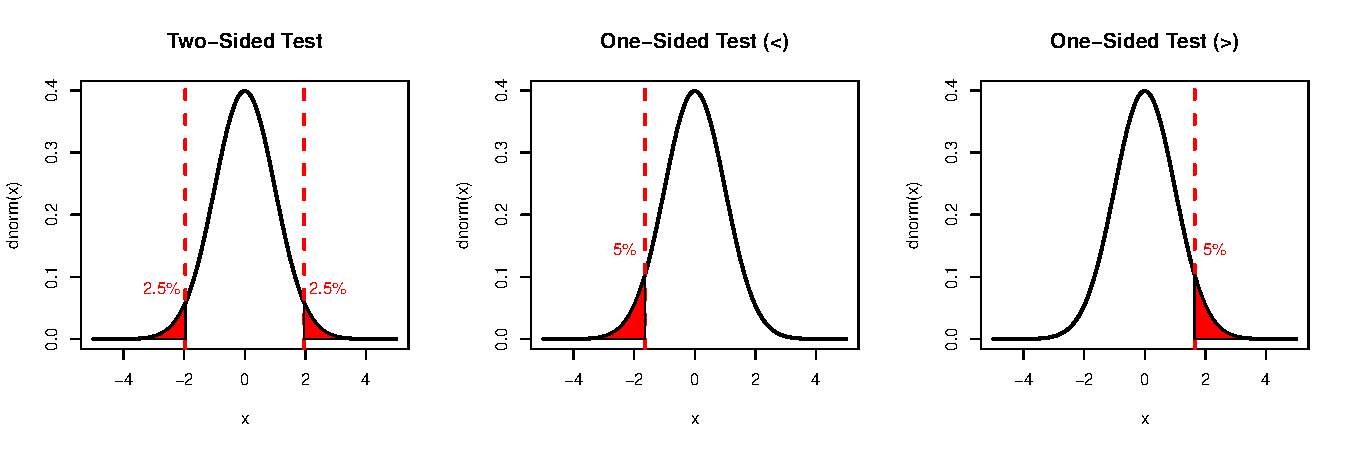
\includegraphics[scale=0.5]{./images/onesided_vs_twosided.pdf}
  \end{figure}

  \vspace{-2em}

  \begin{block}{Two-Sided}
    Splits $\alpha=0.05$ between two tails: $c = \texttt{qnorm}(1 - 0.05/2) \approx 1.96$ 
  \end{block}

  \begin{block}{One-Sided}
    One tail: $c = \texttt{qnorm}(0.05)\approx  -1.64$ for ($<$); $\texttt{qnorm}(0.95) \approx 1.64$ for ($>$) 
  \end{block}
\end{frame}
%%%%%%%%%%%%%%%%%%%%%%%%%%%%%%%%%%%%%%%%
\begin{frame}
  \frametitle{Example: $X_1, \dots, X_{100} \sim \mbox{iid N}(\mu,1), \alpha = 0.05$}

  \small

  \[\boxed{\mbox{Suppose } \bar{x} = 1.5 \implies (\bar{x} - 2)/0.3 \approx -1.67}\]


  \pause

  \begin{columns}
    \column{0.32\textwidth}
    \begin{block}{Two-sided}
      $H_1\colon \mu \neq 2$\\
      Reject if $T_n > 1.96$\\
      $T_n = 1.67$\\
      \alert{Fail to reject}
    \end{block}
    \column{0.32\textwidth}
    \begin{block}{One-sided $(<)$}
      $H_1\colon \mu < 2$\\
      Reject if $T_n < -1.64$\\
      $T_n = -1.67$\\
      \textcolor{blue}{Reject}
    \end{block}
    \column{0.32\textwidth}
    \begin{block}{One-sided $(>)$}
      $H_1\colon \mu > 2$\\
      Reject if $T_n > 1.64$\\
      $T_n = -1.67$\\
      \alert{Fail to reject}
    \end{block}
  \end{columns}

  \pause

  \vspace{2em}
  \begin{itemize}
    \item If One-sided $(<)$ rejects, then one-sided $(>)$ doesn't and vice-versa. \pause
    \item Two-sided and one-sided sometimes agree but sometimes disagree. \pause
    \item One-sided test is ``less stringent.''
  \end{itemize}
  
\end{frame}
%%%%%%%%%%%%%%%%%%%%%%%%%%%%%%%%%%%%%%%%
\begin{frame}
  \frametitle{Testing $H_0\colon \mu = \mu_0$ when $X_1, \dots, X_n \sim \mbox{iid N}(\mu, \sigma^2)$}

  \begin{block}{Two-Sided}
    Reject $H_0$ whenever $\displaystyle \left|\frac{\bar{X}_n - \mu_0}{\sigma/\sqrt{n}}\right|> \texttt{qnorm}(1 - \alpha/2)$ 
  \end{block}

  \begin{block}{One-Sided $(<)$}
    Reject $H_0$ whenever $\displaystyle \frac{\bar{X}_n - \mu_0}{\sigma/\sqrt{n}} < \texttt{qnorm}(\alpha)$ 
  \end{block}

  \begin{block}{One-Sided $(>)$}
    Reject $H_0$ whenever $\displaystyle \frac{\bar{X}_n - \mu_0}{\sigma/\sqrt{n}} > \texttt{qnorm}(1 - \alpha)$ 
  \end{block}


\end{frame}
%%%%%%%%%%%%%%%%%%%%%%%%%%%%%%%%%%%%%%%%
\begin{frame}
  \frametitle{One-sided P-value}

  \small

  \begin{itemize}
    \item Only makes sense to calculate one-sided p-value when sign of test stat.\ agrees with alternative: \pause
      \begin{itemize}
        \item Preceding example: $T_n = -1.67$  \pause
        \item Calculate p-value for test vs.\ $H_1\colon \mu < 2$ but \alert{not $H_1\colon \mu >2$} \pause
      \end{itemize}
    \item Just as in two-sided test, p-value equals value of $\alpha$ for which $c$ exactly equals the observed test statistic: \pause
      \begin{itemize}
        \item $c = \texttt{qnorm}(\alpha)$ for $(<)$ \pause
        \item $c = \texttt{qnorm}(1 - \alpha)$ for $(>)$ \pause
        \item Example: $-1.67 = \texttt{qnorm}(\alpha) \iff \alpha = 0.047$ \pause
      \end{itemize}
    \item Use and report  one-sided p-value in same way as two-sided p-value
  \end{itemize}


\end{frame}
%%%%%%%%%%%%%%%%%%%%%%%%%%%%%%%%%%%%%%%%
\begin{frame}
  \frametitle{Final Notes on One-sided vs.\ Two-sided Tests}

  \begin{itemize}
    \item Two-sided test is the default. \pause
    \item Don't use one-sided unless you have a good reason! \pause
    \item Relationship between CI and test \alert{only holds for two-sided}.\pause
    \item Why and when should we consider a one-sided test?\pause
      \begin{itemize}
        \item Suppose we know \emph{a priori} that $\mu < 2$ is crazy/uninteresting\pause
        \item Test of $H_0\colon \mu=2$ against $H_1\colon \mu>2$ with significance level $\alpha$ has \alert{lower type II error rate} than test against $H_1\colon \mu\neq 2$. \pause
      \end{itemize}
    \item If you use a one-sided test you \alert{must choose $(>)$ or $(<)$ \emph{before looking at the data}}. Otherwise the results are invalid.
  \end{itemize}
\end{frame}
%%%%%%%%%%%%%%%%%%%%%%%%%%%%%%%%%%%%%%%%
\begin{frame}
  \frametitle{Roadmap}
  \small

  \begin{block}{Next Time}
    More examples of hypothesis testing using relationship to CIs to help us avoid re-inventing the wheel.
  \end{block}


  \pause

  \begin{block}{Building Intuition}
   Now that you know a simple example of a hypothesis test and its relationship to a CI, think about the following:
   \begin{itemize}
     \item If we reject $H_0$ does that mean that $H_0$ is false?
     \item How does testing relate to random sampling?
      \item How does critical value of two-sided test relate to width of CI?
      \item In a given test, which is larger: the one-sided or two-sided p-value?
   \end{itemize}
  \end{block}

\end{frame}
%%%%%%%%%%%%%%%%%%%%%%%%%%%%%%%%%%%%%%%%
